\documentclass[main.tex]{subfiles}

\begin{document}

\section{Comparison} \label{sec:comparison}

Given that \hetplats can suffer major changes in the future, due to the constant technological evolution, a highly important feature of an application or framework is its modularity, so that individual features can be updated to meet the requirements of the constantly evolving computing platforms. \starpu seems to use this philosophy to some extent, with modules such as the scheduler itself being completely unpluggable and rewritable by a developer. It also provides the ability to assign user defined functions to make decisions within the framework, such as how to partition data.

\subsection{Usability}

From a developer's point of view, \starpu, being written in $C$ provides an a clear but somewhat outdated API, in some aspects resembling \texttt{UNIX}-like libraries. More modern languages such as $C++$, in which \gama is written provide less verbose and more structured code. The choice for the $C$ language is possibly related to better compatibility and portability, but seems to somewhat limit the language, and even expose some unexpected behaviours of the framework (see \cref{sec:comparison:type_safety,sec:comparison:consistency}).

Even though \gama does not yet provide a solid API to work from, but rather a more confusing architecture, it can still be considered harder to work on, although there is plenty of room for improvement, and once development advances, and reaches a more stable position, it can have the conditions to be a much more usable framework than the low-level one provided by \starpu

\subsection{Scheduling}

Both \starpu and \gama employ a variant of the \acs{HEFT} algorithm for scheduling on heterogeneous systems, although \starpu gives much more emphasis to the latency caused by memory transactions, and can also support additional scheduling policies to be used.

\subsection{Memory Management}

\gama has the ability of recursively changing the granularity of a task to adapt it to the characteristics of a device. This is presented as an important step by \gama to automate decisions by the scheduler. Without this, granularity has to be manually defined, by subdividing the domain in arbitrarily sized chunks and process each one as an individual task. This is not only a cumbersome task for the developer, but also a possible weakness, as the ideal task granularity is not equal from system to system, or algorithm to algorithm, and may not be easy to determine without intensive testing and manual tuning.

This seems an extremely important feature in \gama, at least from the usability point of view, as the task of finding the ideal granularity is thus automated by the framework.

\subsubsection{Type Safety} \label{sec:comparison:type_safety}

Perhaps one of the most important limitations of \starpu's API is the fact that its task submission methods are not type-safe\footnote{the extent to which a language discourages or prevents type errors}. By definition, the C language (in which \starpu is implemented and exposed to the programmer) is by only type safe to a certain extent, since workarounds are often used in the language to achieve results similar to polymorphism or runtime casting.

This is the case with \starpu, resulting in an API that can be mistakenly used by the programmer. Each codelet defined in a program specifies how many data buffers its tasks will depend on, and their access modes. However, since data buffers are used only through their data handles, which are completely generic, no explicit type checking is made to ensure that the correct types of data handles is passed, and that they are received properly within the task. For example, a task may be expecting to receive buffers X and Y of completely different sizes and types. But on task submission, their order might be reversed, resulting in runtime errors which might be extremely difficult to trace.

The main result of this is a weak task submission API, since it can easily lead to runtime errors. More experienced developers might have enough understanding to easily identify these problems. But technical issues such as type safety should not have to be addressed by the developer, as they can pose serious problems to development time, but could be easily identified by a compiler.

\subsubsection{Consistency} \label{sec:comparison:consistency}

\starpu ensures consistency of all data assigned to it via data handles, but only within managed managed by its scheduler. The issue here is that, while the API allows the creation of a data handle associated with an already allocated data structure (usually pinned to main system memory), it is not ensured that tasks will write to that actual memory, and not a \starpu-managed copy. This has the side effect of consistency not being ensured outside of the context of a task. Writing to a buffer via conventional methods can thus be considered dangerous.

It is also impossible to change the size of a data buffer once it has been assigned to \starpu. When this is a requirement, is to destroy and redefine the buffer, which is not a particularly efficient method, and may introduce additional bottlenecks when used between task submissions.

On these subjects, \gama seems to provide more powerful capabilities. All data that is to be managed by \gama's unified memory system must be encapsulated in a wrapper that processes all accesses to it. While it is not documented how \gama actually behaves when data is accessed outside of a job, this model should provide a more transparent solution for consistent memory access.


\subsubsection{Data Access Modes}

Another caveat of the usage of data handles is that it can lead to incoherent results, again due to possible and easily made developer mistakes. \starpu relies on the estimation of data transfer times to decide where to schedule a task to. An important factor of this comes from the access modes required for each data buffer in a task, as explained in \cref{sec:starpu:data_access}.

If a data buffer is declared as read-only within a task, it is assumed to be unchanged by that same task, this other tasks depending on it have that dependency already met.
The caveat here is that a read-only buffer is only so for the framework, but not actually read-only for the programmer, or for the C compiler itself, and data can actually be overwritten for a read-only buffer. Although that is probably related to a development mistake, it can easily happen nonetheless

Adding to this is the fact that \starpu might create additional copies of data buffers to solve dependencies faster across multiple devices. \cref{fig:deps_problem} exemplifies this problem. Tasks A and B have read-only access to the data buffer $x$, although as explained, both of them can write to it at will. If both tasks are scheduled to the same device (\cref{fig:deps_problem:a}, they will be executed in order, and \starpu will reuse the initially existing memory, without the need to create temporary copies of the buffer. In this case, if task A writes to $x$, task B will later see these changes, since memory is shared.


\begin{figure}[!htp]
  \centering
  \begin{subfigure}{.5\textwidth}
    \centering
    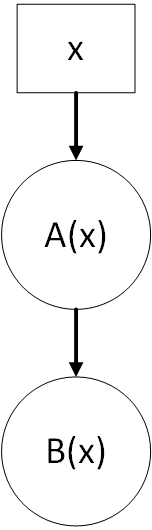
\includegraphics[width=0.2\linewidth]{visio/starpu_dep_rw}
    \caption{A and B are executed in order \label{fig:deps_problem:a}}
  \end{subfigure}%
  \begin{subfigure}{.5\textwidth}
    \centering
    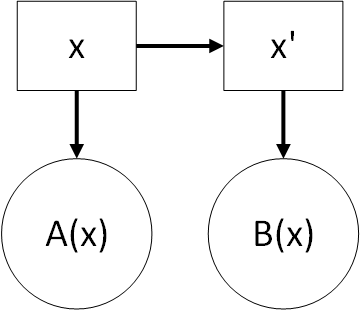
\includegraphics[width=0.6\linewidth]{visio/starpu_dep_rw_caveat}
    \caption{A and B are scheduled to different devices, creating a temporary copy of $x$, and running both tasks concurrently \label{fig:deps_problem:b}}
  \end{subfigure}
  \caption{Illustration of a possible mistake due to dependency management. Both A and B have read-only access to $x$ \label{fig:deps_problem}}
\end{figure}

In \cref{fig:deps_problem:b}, the two tasks are scheduled to different devices. Since \starpu assumes $x$ to be read-only, a copy of it, $x'$ can immediately be created in the additional device. In this case, both tasks will run concurrently, with their own local copy of $x$. Task A will still write changes to this buffer, but task B will not see them.

\end{document}
